\documentclass[../ClipsManualeUtente.tex]{subfiles}

\begin{document}
\section{Per iniziare: Navigazione indoor}
	Per iniziare ad utilizzare subito l'applicazione e navigare nell'edificio di tuo interesse:
	\begin{enumerate}
		\item attiva il \textbf{bluetooth}. Altrimenti all'avvio l'applicazione ti chiederà il permesso di attivarlo (figura \ref{fig:AvvisoBLE});
		\item attiva una \textbf{connessione dati} oppure una \textbf{connessione Wi-fi} e assicurati che lo smartphone sia connesso ad Internet;
		\item \textbf{avvia l'applicazione} selezionando l'icona 
\includegraphics[scale=0.4]{img/LogoApp};
		\item assicurati di essere in un \textbf{edifico supportato} dall'applicazione. Per assicurarsi di ciò basta accertarsi che dalla schermata principale dell'applicazione siano visibili le informazioni dell'edificio;
		
		\begin{framed}
			\textbf{Nota:} solo per i dispositivi con \textbf{Android `Marshmallow' 6.0} - il \textbf{GPS} dello smartphone deve essere \textbf{attivato} prima di avviare l'applicazione. Se non è attivo all'avvio l'applicazione chiederà il permesso di attivarlo come mostrato in figura \ref{fig:AvvisoGPS}.
		\end{framed}
		
		\item nella schermata principale (figura \ref{fig:HomeApp}), se l'edificio è stato identificato, potrai trovare:
		\begin{itemize}
			\item informazioni relative all'edificio: nome, indirizzo e una breve descrizione dell'edificio;
			\item orari di apertura e chiusura dell'edificio;
			\item una lista di categorie che raccolgono tutte le possibili aree d'interesse da raggiungere;
		\end{itemize}
		\item dalla lista sotto: \textit{`La Struttura'} mostrata in figura \ref{fig:CategoriePoi} seleziona la categoria di tuo interesse;
		
		\begin{figure} [p]
			\centering
			\subfloat[][Avviso mostrato nel caso il Bluetooth sia spento]
			{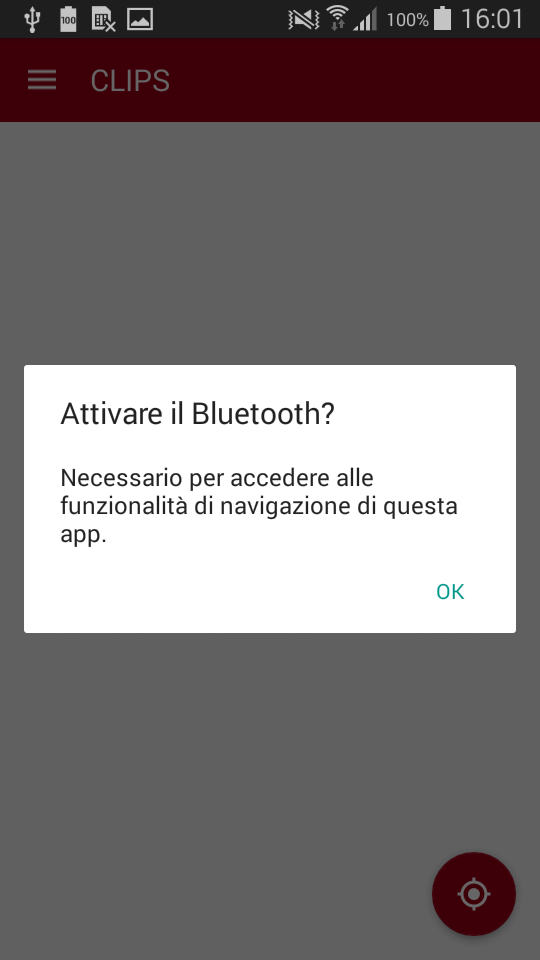
\includegraphics[width=.33\textwidth]{img/AvvisoBLE}
			\label{fig:AvvisoBLE}} \quad
			\hspace{1.5cm}
			\subfloat[][Avviso mostrato nel caso il GPS sia spento]
			{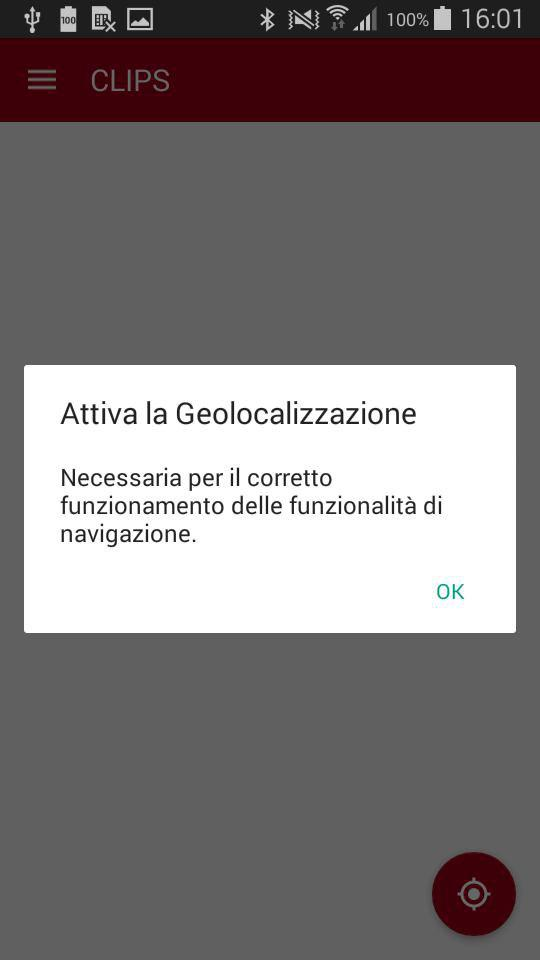
\includegraphics[width=.33\textwidth]{img/AvvisoGPS}
			\label{fig:AvvisoGPS}} \\
			
			\subfloat[][Schermata principale dell'applicazione che riporta le informazioni dell'edificio in cui ci si trova]
			{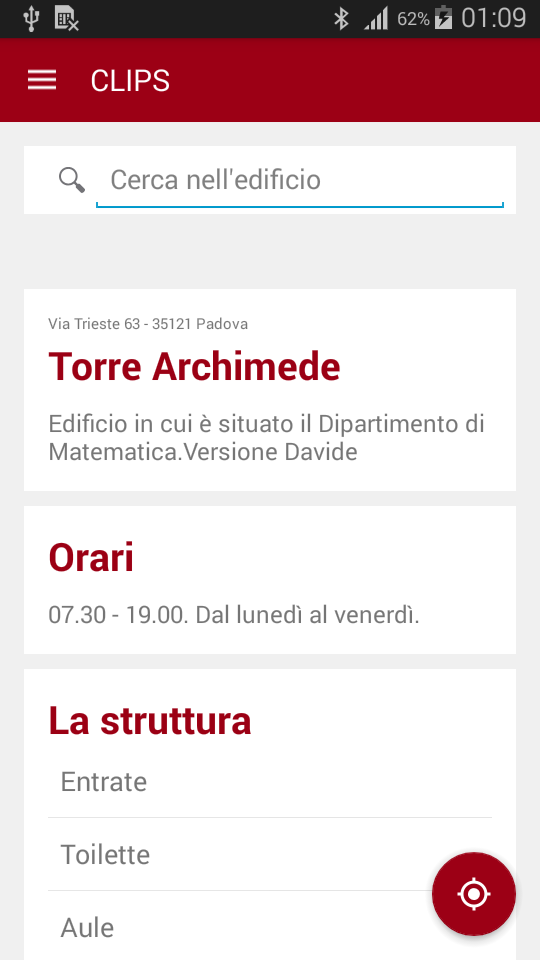
\includegraphics[scale=0.33]{img/HomeApp}
			\label{fig:HomeApp}} \quad
			\hspace{1.5cm}
			\subfloat[][Zoom sulla lista di categorie delle possibili destinazioni]
			{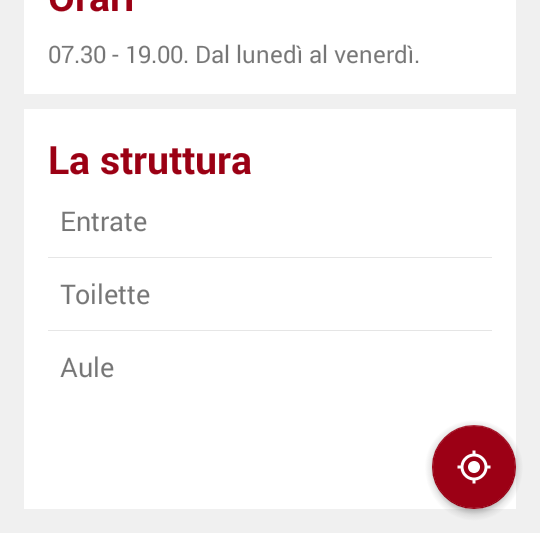
\includegraphics[scale=0.33]{img/CategoriePoi}
			\label{fig:CategoriePoi}} \\
			\caption{Avvisi mostrati all'avvio dell'applicazione e Schermata principale dell'applicazione}
		\end{figure}
			
			
		\newpage	
		
		\item si aprirà una schermata simile a quella in figura \ref{fig:ListaPoi}, ora puoi selezionare l'area d'interesse che vuoi raggiungere;
		\item segui le indicazioni mostrate per raggiungere l'area scelta precedentemente (figura \ref{fig:ListaIstruzioni}).
				
	\end{enumerate}
		
		\begin{figure} [h]
			\centering
			\subfloat[][Lista delle possibili destinazioni della categoria \textit{`Aule'}]
			{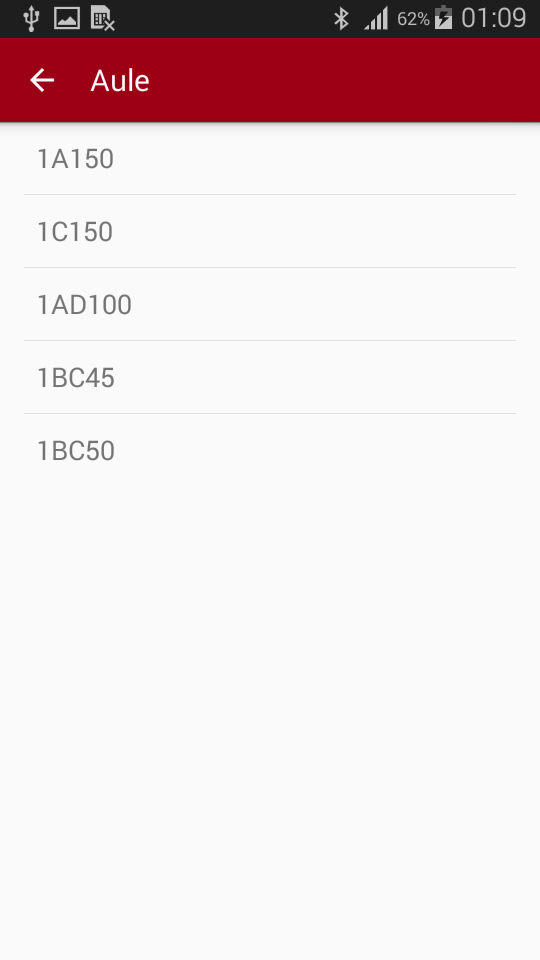
\includegraphics[width=.33\textwidth]{img/ListaPoi}
			\label{fig:ListaPoi}} \quad
			\hspace{1.5cm}
			\subfloat[][Lista di istruzioni da seguire per raggiungere la destinazione scelta]
			{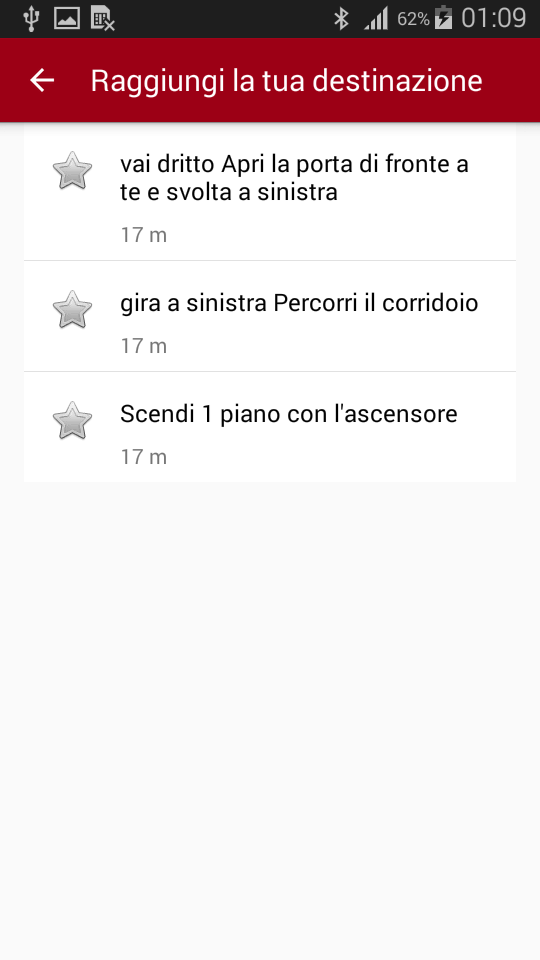
\includegraphics[width=.33\textwidth]{img/ListaIstruzioni}
			\label{fig:ListaIstruzioni}} \\
			\caption{Cominciare una navigazione}
		\end{figure}				
	

\end{document}